\documentclass[a4paper, 12pt]{article}
\usepackage{comment} % enables the use of multi-line comments (\ifx \fi)
\usepackage{fullpage} % changes the margin
\usepackage{enumitem}
\usepackage{graphicx}
\usepackage{hyperref}
\usepackage{wrapfig}


\begin{document}
%Header-Make sure you update this information!!!!
\noindent
\large\textbf{Visual Analytics - Final Project} \normalsize \hfill Due Date: 10/06/2018 \\
\normalsize Engineering in Computer Science   \\
Prof. Giuseppe Santucci \hfill Valerio Colitta - 1656690 \\
TA: Marco Angelini \hfill Davide Spallaccini - 1642557

\section*{Flights And Delays In The United States}

\paragraph{Introduction}
The airline industry is one of the fields that continuously produces a large amount of complex data
regarding the large number of flights that take place every day. In this work we concentrate only on
flights of a single year in the United States. Even considering a single nation and a single year the
number of flights is really high, so in this work we aim at providing a visualization of this data that
helps in better understanding patterns in the number of flights in the different states and in the 
delays that were recorded across time.

\paragraph*{Data}
We got our data from the United States Department of Transportation, and in particular from the 
Bureau of Transportation Statistics (BTS) website. As the independent statistical agency within the
Department of Transportation (DOT), the Bureau of Transportation Statistics (BTS) is a politically
objective supplier of trusted and statistically sound baseline, contextual, and trend information used
to shape transportation policy, investments, and research across the U.S. and abroad. BTS is the
preeminent source of statistics on commercial aviation, and transportation economics.
In particular we used the On-Time Performance table (available at ...) under the Airline and Airports
subsection of the website. This table contains on-time arrival data for non-stop domestic flights by
major air carriers, and provides such additional items as departure and arrival delays, origin and
destination airports, flight numbers, scheduled and actual departure and arrival times, cancelled or
diverted flights, taxi-out and taxi-in times, air time, and non-stop distance.\\ \\
It is a very large dataset, that contains more than \texttt{5 millions} records of flights in the United States. The main features are:
\begin{itemize}
	\item \texttt{ARR\_DELAY} : minutes of delay on the arrival for the flight 
	\item \texttt{DEP\_DELAY} : minutes of delay on the departure for the flight
	\item \texttt{AIR\_TIME} : minutes of air-time
\item \texttt{DISTANCE} : distance in miles covered by the airplane
\item \texttt{CARRIER\_DELAY} : Carrier delay in minutes  
\item \texttt{NAS\_DELAY}: National Air System delay, in minutes
\item \texttt{LATE\_AIRCRAFT\_DELAY} : Late aircraft delay in minutes
\item \texttt{ORIGIN\_STATE\_ABR} : State of departure abreviation
\end{itemize}
Because of the huge amount of data, we couldn't just load them via d3 or javascript; we tried, but the time to load it was just too much. Therefore we decided to do some preprocessing on the data, before loading them.\\
Flights were grouped by \texttt{month, state} and counted to use those values in the \texttt{USA map}. The same happened for the \texttt{DD scatter plot}\\ \\
In addition to that, we randomly sampled about a thousand records, in order to plot the single instances on the parallel coordinates, and perform the PCA on them.

\paragraph*{State Patterns}
The first visualization elements we are going to describe have the goal to display for each state the 
amount of airline departures. In particular we want to visualize how many flights leave each state during
the different months of the year and how these numbers vary from state to state. For the first task we
drew a map of the USA and colored each state according to the number of flights for the selected month
with a heat map. The color of each state in this case is independent from the color of the other states,
it only depends on the mean of flights for that state during the year. A \emph{hot} color tells that in
that month the number of flights was higher than the average while a \emph{cold} color that the number of
flights was respectively low. A slider under the map allows the user to change the month under
consideration. On the other hand, in order to visualize how the number of flights differs from state to 
state in a quantitative fashion we display a bar chart with a bar for each state whose height is
proportional to the number flights in that state. When you click on a bar the bar becomes red and a line
appears cutting all the other bars at the height of the selected one, highlighting the differences; if 
then you over the mouse on other bars the difference number (positive or negative) is shown.

We found interesting that some patterns appear really clear in the map, for example in February almost
everywhere the number of flights is below the average, on the contrary in August this number is far over
the average probably highlighting the departures due to holidays. In July the same observations hold, and 
in particular northern countries tend to have higher increase of flights. An exception to the summer 
excitement is Florida, probably because it is one of the destination for holiday travels and local
population usually stays in the country.\\
\begin{figure}[h]
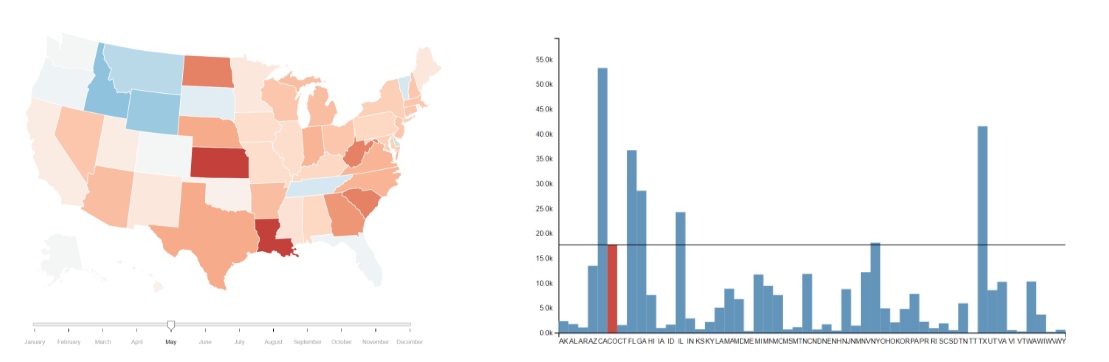
\includegraphics[scale=0.7]{usamapbar.PNG}
\end{figure}\\
\paragraph*{Delays}
The other visualization elements we devised concern flights delays.\\
We created three views:
\begin{itemize}
\item \texttt{PCA plot}
\item \texttt{Parallel Coordinates}
\item \texttt{DD scatter}
\end{itemize}
\subparagraph{PCA plot} This plot displays in 2D the records sampled in the dataset. In order to project them in 2D we applied PCA via a python script.\\
Out of all the sampled elements we took only the ones that had some delay at the arrival or at the departure.\\
\begin{wrapfigure}{l}{0.54\textwidth}
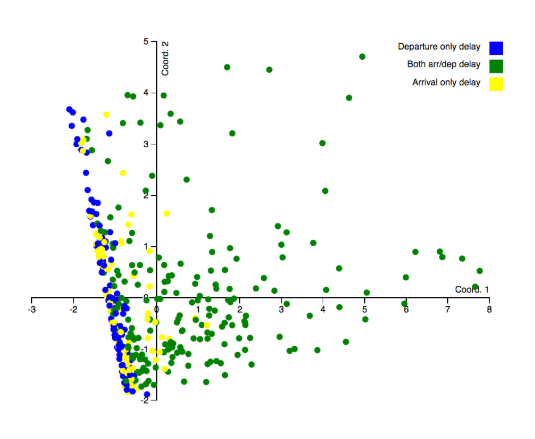
\includegraphics[scale=0.7]{pca.PNG}
\end{wrapfigure}\\ 
Once plotted we categorized them in three classes (\texttt{Departure delay only, Arrival delay only,\\ Both Arrival/Departure delay}).\\
An interesting result, was to notice that flights form clusters, and thus there is a good chance that they are close each other also in higher dimensions.\\ \\ \\ \\ \\
\subparagraph{Parallel Coordinates}The same data used in the PCA plot were used in the parallel coordinates. PC are a standard method to visualize high dimensions on a 2D environment. For this view we decided to use almost only numeric features that concerned delays. This was made because they were the only numeric values available.\\
\begin{figure}[h]	
\centering
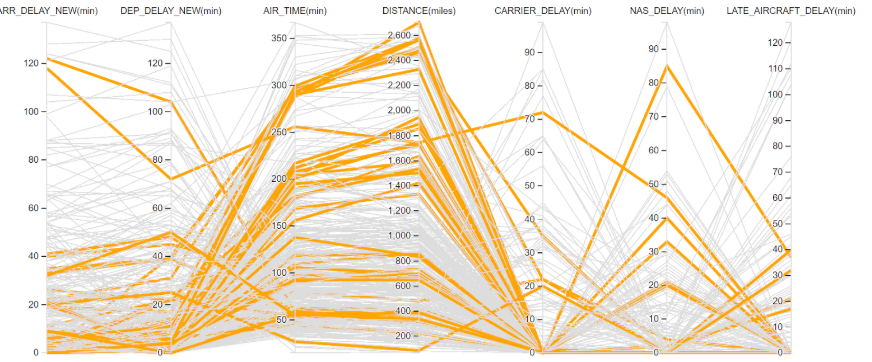
\includegraphics[scale=0.7]{pc.PNG}
\end{figure}\\
To give a better user-experience, axis can be moved around and interval of interests can be selected.\\
This view is also coordinated with the USA map. Whenever we want to know what are the flights departed from one of the states, we can filter those by clicking on the state in the map. The lines regarding these flights will be highlighted in orange.
\subparagraph{DD scatter} The last view in the second group is the DD scatter. It displays relationships between flight delays and their distances.
We decided to use a scatter plot where on the x-axis there are all the possible intervals of distance, while on the y-axis the intervals for the delays. Each cell represents the \texttt{number of flights whose distances and delays lie in that intervals}.\\
It is colored according to a heatmap, in order to distinguish the quantities.\\ \\
\begin{figure}[h]	
\centering
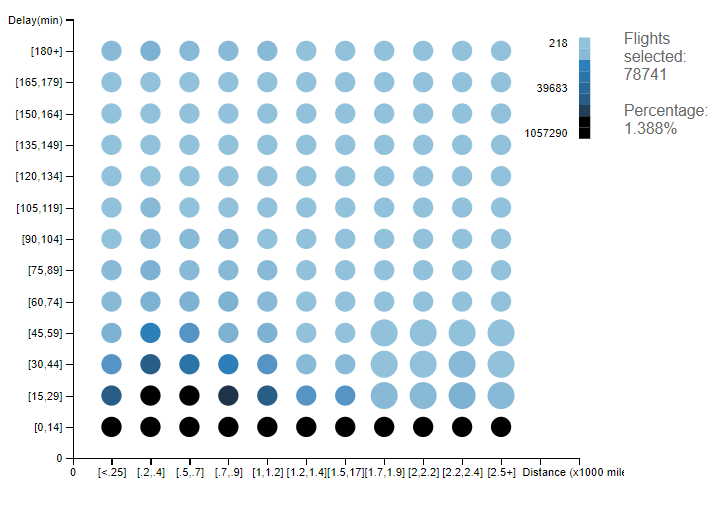
\includegraphics[scale=0.7]{ddscat.PNG}
\end{figure}\\
Group of point can be selected, and the exact number, together with the percentage out of all flights they occupy is displayed. This is useful in order to "query" the dataset. For example, thanks to this view, we noticed that during the whole year of 2017, the number of flights that did not delayed more than 15 minutes is the 81\%, while those for which the delay was greather than \texttt{three hours} are just the 1\%, that means about 60.000 flights.\\
Another data extracted thanks to this view, is that most of the flights tend to cover about 500 - 1000 miles.\\\\
Lastly we notices that the delays tend to decrease with the increase of the flight's distance. 
\paragraph{Why using a scatter plot ?}
We opted for this, over a correlation matrix for two main reasons. First, it works on two different features and then it is not symmetric. A correlation matrix is symmetric.\\
Second reason, we wanted it to brushable, to have some interaction with it. In a correlation matrix this would be possible, but in a limited way



\paragraph*{Conclusions}

(Slides for this project are available \href{https://docs.google.com/presentation/d/1T_p1oarqUuNt5APTaf7IwTJEzUDJC0CoNfJKHdak0so/edit?usp=sharing}{here}).


\end{document}
